
\documentclass{article}
\usepackage[a4paper, portrait, margin=1.1811in]{geometry}
\usepackage[english]{babel}
\usepackage[utf8]{inputenc}
\usepackage[T1]{fontenc}
\usepackage{helvet}
\usepackage{etoolbox}
\usepackage{graphicx}
\usepackage{titlesec}
\usepackage{caption}
\usepackage{booktabs}
\usepackage{xcolor} 
\usepackage[colorlinks, citecolor=cyan]{hyperref}
\usepackage{caption}
\captionsetup[figure]{name=Figure}
\graphicspath{ {./images/} }
\usepackage{scrextend}
\usepackage{fancyhdr}
\usepackage{graphicx}
\newcounter{lemma}
\newtheorem{lemma}{Lemma}
\newcounter{theorem}
\newtheorem{theorem}{Theorem}

\fancypagestyle{plain}{
	\fancyhf{}
	\renewcommand{\headrulewidth}{0pt}
	\renewcommand{\familydefault}{\sfdefault}
	
	\lhead{\color{cyan}\small \textbf{Journal of Aerosol Science}\\ \color{black}
	\textit{Vol. XX (X)  (XXXX), XX-XX, p-ISSN: 693-7554, e-ISSN:2654-3990}\\ }
	%\rhead{p-ISSN: 693-7554 \\ e-ISSN:2654-3990}
	%\rfoot{\thepage} --> Show the page number
	
}

%\pagestyle{plain}
\makeatletter
\patchcmd{\@maketitle}{\LARGE \@title}{\fontsize{16}{19.2}\selectfont\@title}{}{}
\makeatother

\usepackage{authblk}
\renewcommand\Authfont{\fontsize{10}{10.8}\selectfont}
\renewcommand\Affilfont{\fontsize{10}{10.8}\selectfont}
\renewcommand*{\Authsep}{, }
\renewcommand*{\Authand}{, }
\renewcommand*{\Authands}{, }
\setlength{\affilsep}{2em}  
\newsavebox\affbox
\author[1]{\textbf{João P. M. Marques}}
\author[2]{\textbf{Luewton F. L. Agostinho}}
\author[3]{\textbf{Antonio Carrasco}}
\author[4*]{\textbf{Fourth author}}
\affil[1,2]{ Study Program, Faculty, University
	Bogor, West Java, 16143, Indonesia
}
\affil[3]{ Department of Computer Science, Faculty of Mathematics and Natural Science, Pakuan University, 
	Bogor, West Java, 16143, Indonesia
}
\affil[4]{ Department of Mathematical Sciences, Faculty of Science,
	Universiti Teknologi Malaysia,
	81310 Johor Bahru,
	Johor, Malaysia
}

\titlespacing\section{0pt}{12pt plus 4pt minus 2pt}{0pt plus 2pt minus 2pt}
\titlespacing\subsection{12pt}{12pt plus 4pt minus 2pt}{0pt plus 2pt minus 2pt}
\titlespacing\subsubsection{12pt}{12pt plus 4pt minus 2pt}{0pt plus 2pt minus 2pt}


\titleformat{\section}{\normalfont\fontsize{10}{15}\bfseries}{\thesection.}{1em}{}
\titleformat{\subsection}{\normalfont\fontsize{10}{15}\bfseries}{\thesubsection.}{1em}{}
\titleformat{\subsubsection}{\normalfont\fontsize{10}{15}\bfseries}{\thesubsubsection.}{1em}{}

\titleformat{\author}{\normalfont\fontsize{10}{15}\bfseries}{\thesection}{1em}{}

\title{\textbf{\huge EHDA closed loop control system based on real time non-visual spray mode classification}\\
	(Center, Bold, Times New Roman 14, maximum 15 words in english)}
\date{}    

\begin{document}

\pagestyle{headings}	
\newpage
\setcounter{page}{1}
\renewcommand{\thepage}{\arabic{page}}


	
\captionsetup[figure]{labelfont={bf},labelformat={default},labelsep=period,name={Figure }}	\captionsetup[table]{labelfont={bf},labelformat={default},labelsep=period,name={Table }}
\setlength{\parskip}{0.5em}
	
\maketitle
	
\noindent\rule{15cm}{0.5pt}
	\begin{abstract}
		\textbf{Electrohydrodynamic Atomization (EHDA)} also known as Electrospray (ES), is a technology that uses a strong electric field (kV/cm) to manipulate liquid breakup into droplets. This technique allows the generation of droplets smaller than the nozzle diameter with a controlled droplet size, which means it can be used to produce uniformly sized particles in the micro/nanoscale range. This liquid spraying technique can generate different modes when both the liquid flow rate and the voltage vary with a narrow size dispersion. The most known mode is the cone-jet mode, because it can produce droplets in the micro and nanometric range with a narrow size dispersion.
		The article presents a novel closed-loop control system for electrohydraulic actuators (EHDA) that utilizes real-time, non-visual spray mode classification to improve performance and efficiency. The system utilizes current data from the experiment to classify the spray mode dynamics in real-time and adjust the EHDA parameters, such as pump flowrate and power supply voltage, to reach the desired spray mode and stabilize it. The proposed control algorithm is able to achieve improved accuracy and reduced waste compared to previous methods. The results of the system are discussed and its potential applications in industrial settings are highlighted.
		consists of objectives, methods, findings, and research contributions in 150 to 250 words which contains the main conclusions and provides important information and is accompanied by \textbf{5 keywords}. Furthermore, the determination of keywords needs to pay attention to important words contained in the title and abstract, separated by a semicolon. \textbf{The novelty} in this paper briefly explains why no one else has adequately researched the question. Then \textbf{the results} are made a list of the empirical findings and write the discussion in one or two sentences. \\ \\
		\let\thefootnote\relax\footnotetext{
			\small $^{*}$\textbf{Corresponding author.} \textit{
				\textit{E-mail address: \color{cyan}author4@email.com}}\\
			\color{black} Received: xx xxxxx 20xx,\quad
			Accepted: xx xxxxx 20xx and available online XX July 2022 \\
			\color{cyan} https://doi.org/10.1016/j.compeleceng.2021.107553
			
		}
		\textbf{\textit{Keywords}}: \textit{Keyword 1; keyword 2; keyword 3; keyword 4; keyword 5}
	\end{abstract}
\noindent\rule{15cm}{0.4pt}

\section{Introduction (10pt, bold)}
The introduction is about 400-600 words and provides background information, previous references related to the main topic, reason, purpose of the research, and the novelty of the research.  Content should be relatively non-technical, but clear enough for a knowledgeable reader to understand the manuscript’s contribution. Explain what the purpose of the research is and why the research was conducted the main body of the article should begin with an introduction, which provides further details on the purpose of the paper, motivation, research methods, and findings. For citations use numbering which must be used for reference titles, for example, citations for journals consisting of 1 article  \cite{Septiawan1} or two articles \cite{Septiawan2}, \cite{Lucy}, while for writing citations of more than two articles \cite{Gingold} - \cite{Morikawa}.

In writing a bibliography using the IEEE style, the conditions are numbered, as follows: \cite{Septiawan1}, in order from the first citation to the last. References with IEEE style use a numeric number placed in a square box for the reference taken and put it at the end of the sentence. The numeric numbers located in the square box are made the same as the bibliography on the final page of the scientific paper.

\section{Methods (10pt, bold)}
The methods section describes the steps followed in the execution of the study and also provides a brief justification for the research methods used. A chronological explanation of the research, including research design, research procedures (in the form of algorithms, codes, or others), how the procedures are to obtain and test data \cite{Lo} - \cite{Hang}. The description of the research has been supported by references, so that the implementation can be accepted scientifically [6]. Figure are presented in the center, as shown below and are cited in the manuscript. An example of a membership function graph can be seen in Figure \ref{table1}.

\begin{figure}[h]
	\centering
	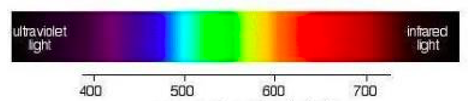
\includegraphics[width=0.5\textwidth]{images/figur1.PNG}
	\caption{Font 10pt and center not bold for captions except for the words "Figure"}
	\label{fig1}
\end{figure}

Each image (photos, graphs, and diagrams) in the article must be accompanied by a caption/image title and sequential image numbers, written below the image in the middle position. Images must be directly relevant to the article and are always referenced in the article referred to as Figur \ref{table1}, where the capital letters are capitalized.

\subsection{Table (10pt, bold)}
Writing tables are numbered followed by the title of the table above the table, centered, 1 spaced with a short and precise title. Consider the example in Table \ref{table1}
\begin{table}[h]
	\centering
	\caption{Font 10pt and center not bold for captions except for the words "Table"}
	\label{table1}
	\begin{tabular}{@{}cccc@{}}
		\toprule
		\textbf{Characteristics}& \textbf{Description }& \textbf{Frequency }& \textbf{Percentage} \\
		\midrule
		Gender & Male & 198 & 80.2\% \\
		& Female & 49 & 19.8\% \\
		Entry & 2018 & 54 & 21.9\% \\
		& 2019 & 64 & 25.9\% \\
		& 2020 & 59 & 23.9\% \\
		& 2021 & 70 & 28.3\% \\
		MBKM & Yes & 217 & 87.9\% \\
		& No & 30 & 12.1\% \\
		& Total & 247 & 100\% \\
		\bottomrule
	\end{tabular}
\end{table}


\subsection{Figure (10pt, bold)}
Image writing techniques in scientific papers must also be symmetrical in the middle. So the settings are not aligned right or left, but in the center. This helps tidy up the position of the image or photo so that it appears side by side well with the description text as in Figure \ref{fig2}.

\begin{figure}[h]
	\centering
	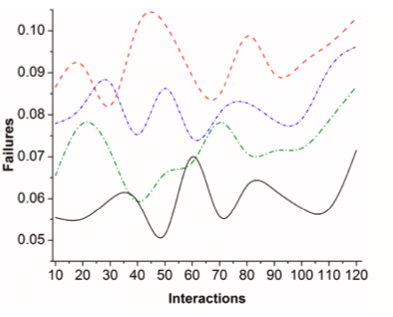
\includegraphics[width=0.5\textwidth]{images/figur2.PNG}
	\caption{Font 10pt and center not bold for captions except for the words "Figure"  }
	\label{fig2}
\end{figure}


\section{Result and Discussion (10pt, bold)}
The results obtained are data or facts obtained from research. Important data or facts that cannot be clearly narrated can be displayed in the form of tables or pictures or other illustrations. If the results are presented in the form of tables or figures, they do not need to be described at length. The discussion is a review of the results, explaining the meaning of the research results, conformity with the results or previous research, the role of the results in solving the problems mentioned in the introduction, and the possibility.

This section is the most important part of your article. The following are things that you must pay attention to in writing the results and the research results must be clear and concise, the data presented has been processed (not raw data), set forth in the form of narratives, tables or pictures, and given easy-to-understand explanations. It is important to highlight differences between your results or findings and those of previous publications by other researchers. It is important to be compared with related references.
\subsection{Equation (10pt, bold)}
Mathematical equations must be numbered sequentially and starting with (1) until the end of the paper including the appendix. This numbering must begin and end with an opening and closing parenthesis and right align. Add one blank space above and below the Eq. \ref{Eq1}.
\begin{eqnarray}
	\chi(L(\Gamma); \lambda)=(\lambda+2)^{m-n}\chi(\Gamma;\lambda+2-k)
	\label{Eq1}
\end{eqnarray}
For example, from Eq. \ref{Eq2} it is derived again the next mathematical equation
\begin{eqnarray}
	\chi(L(\Gamma); \lambda)=\det (\lambda I_{m}-A_{L})
		\label{Eq2}
\end{eqnarray}
Or there is the next mathematical Eq. \ref{Eq3} as below
\begin{eqnarray}
\det(D_{0}D_{0}^{t})=\sum_{|U|=n-1} \det(D_{U})\det(D_{U}^{t})
	\label{Eq3}
\end{eqnarray}
\subsection{Therema (10pt, bold)}
The schema for writing definitions, theorems, lemmas, and proofs conforms to and follows the template below.

\begin{theorem}
	 Theorem is a statement about mathematics that still requires proof and the statement can be shown to have a truth value or is also true.
\end{theorem}

\subsubsection{Lemma (10pt, bold)}
\begin{lemma}
	An entry is a word or phrase entered in the dictionary beyond the definition given in the entry
\end{lemma}

\section{Conclusion (10pt, bold)}
The author presents brief conclusions from the results of research with suggestions for advanced researchers or general readers. A conclusion may review the main points of the paper, do not replicate the abstract as the conclusion. Conclusions must identify the results obtained in a clear and unambiguous manner, the author should provide the answer to the question: is this a problem with error, method, validity, and or otherwise?

\section{Acknowledgement (if any)}
Contains an acknowledgment of thanks to an agency if this research was funded or supported by that agency, or if there were parties who significantly assisted directly in the research or writing of this article. If the party is already listed as the author, then there is no need to mention it again in this Acknowledgment
\bibliographystyle{IEEEtran}

%\bibliography{template} %-->reference list is on the template.bib file
\begin{thebibliography}{1.7} 
	\bibitem[1]{Septiawan1} \color{cyan}R. R. Septiawan, “An ODE control system of a rigid body on an ocean wave for a surfer simulation in the SPH method,” \textit{The Science Reports of Kanazawa University}, vol. 62, pp. 51–68, 2018. [Online]. Available: http://scirep.w3.kanazawa-u.ac.jp/articles/62-004.pdf. \color{black}
	\bibitem[2]{Septiawan2} \color{cyan}R. R. Septiawan, S. Viridi, and Suprijadi, “The Effect of Particle Size Ratio on Porosity of a Particles Deposition Process,” \textit{Key Engineering Materials,} vol. 675–676, pp. 647–650, 2016. [Online]. Available: https://www.scientific.net/KEM.675-676.647. \color{black}
	\bibitem[3]{Lucy} \color{cyan}L. B. Lucy, “A numerical approach to the testing of the fission hypothesis,” \textit{The astronomical journal}, vol. 82, pp. 1013–1024, 1977. \color{black}
	\bibitem[4]{Gingold} \color{cyan}R. A. Gingold and J. J. Monaghan, “Smoothed particle hydrodynamics: theory and application to non-spherical stars,” \textit{Monthly Notices of the Royal Astronomical Society}, vol. 181, no. 3, pp. 375–389, 1977. [Online]. Available:  https://academic.oup.com/mnras/article/181/3/375/988212. \color{black}
	\bibitem[5]{Supriadi} \color{cyan}Suprijadi, F. Faizal, and R. R. Septiawan, “Computational Study on Melting Process Using Smoothed Particle Hydrodynamics,” Journal of Modern Physics, vol. 05, no. 03, pp. 112–116, 2014. [Online]. Available: https://www.scirp.org/pdf/JMP2014022411463120.pdf.\color{black}
	\bibitem[6]{Septiawan3} \color{cyan}R. R. Septiawan, H. Abdillah, Novitrian, and Suprijadi, “Preliminary Study on Liquid Natural Convection by Temperature Differences,” 2015. [Online]. Available: https://www.atlantis-press.com/proceedings/icaet-14/16166.\color{black}
	\bibitem[7]{Morikawa}\color{cyan}D. Morikawa, M. Asai, N. Idris, Y. Imoto, and M. Isshiki, “Improvements in highly viscous fluid simulation using a fully implicit SPH method,” \textit{Computational Particle Mechanics}, vol. 6, no. 4, pp. 529–544, 2019. [Online]. Available: https://link.springer.com/article/10.1007/s40571-019-00231-6.\color{black}
	\bibitem[8]{Lo} \color{cyan}E. Y.M. Lo and S. Shao, “Simulation of near-shore solitary wave mechanics by an incompressible SPH method,” \textit{Applied Ocean Research}, vol. 24, no. 5, pp. 275–286, 2002. [Online]. Available: https://www.sciencedirect.com/science/article/abs/pii/S0141118703000026.\color{black}
	\bibitem[9]{Dalrymple} \color{cyan}R. A. Dalrymple and B. D. Rogers, “Numerical modeling of water waves with the SPH method,” Coastal Engineering, vol. 53, no. 2–3, pp. 141–147, 2006. [Online]. Available: https://www.sciencedirect.com/science/article/abs/pii/S0378383905001304.\color{black}
	\bibitem[10]{Yan} \color{cyan}X. Yan, Y.-T. Jiang, C.-F. Li, R. R. Martin, and S.-M. Hu, “Multiphase SPH simulation for interactive fluids and solids,” ACM Transactions on Graphics, vol. 35, no. 4, pp. 1–11, 2016. [Online]. Available: https://dl.acm.org/doi/10.1145/2897824.2925897.\color{black}
	\bibitem[11]{Antocy} \color{cyan}C. Antoci, M. Gallati, and S. Sibilla, “Numerical simulation of fluid–structure interaction by SPH,” Computers and Structures, vol. 85, no. 11–14, pp. 879–890, 2007. [Online]. Available: https://www.sciencedirect.com/science/article/abs/pii/S0045794907000132.\color{black}
	\bibitem[12]{Monaghan1} \color{cyan}J. J. Monaghan, A. Kos, and N. Issa, “Fluid Motion Generated by Impact,” Journal of Waterway, Port, Coastal, and Ocean Engineering, vol. 129, no. 6, pp. 250–259, 2003. [Online]. Available: https://ascelibrary.org/doi/10.1061/\%28ASCE\%290733-950X\%282003\%29129\%3A6\%28250\%29.\color{black}
	\bibitem[13]{Akinci} \color{cyan}N. Akinci, M. Ihmsen, G. Akinci, B. Solenthaler, and M. Teschner, “Versatile rigid-fluid coupling for incompressible SPH,” ACM \textit{Transactions on Graphics}, vol. 31, no. 4, pp. 1–8, 2012. [Online]. Available: https://dl.acm.org/doi/10.1145/2185520.2185558. \color{black}
	\bibitem[14]{Liu} \color{cyan}G. R. Liu and M. B. Liu, \textit{Smoothed Particle Hydrodynamics}. Singapore: World Scientific Publishing Co Pte Ltd, 2003. doi: 10.1142/5340. \color{black}
	\bibitem[15]{John} \color{cyan}John F. Wendt, \textit{Computational Fluid Dynamics}. Berlin, Heidelberg: Springer Berlin Heidelberg, 2009. doi: 10.1007/978-3-540-85056-4.\color{black}
	\bibitem[16]{Lattanzio} \color{cyan}J. J. Monaghan and J. C. Lattanzio, “A refined particle method for astrophysical problems,” \textit{Astron Astrophys}, vol. 149, pp. 135–143, 1985.\color{black}
	\bibitem[17]{Batchelor}\color{cyan}G. K. Batchelor, \textit{An Introduction to Fluid Dynamics.} Cambridge: Cambridge University Press, 2000. doi: 10.1017/CBO9780511800955.\color{black}
	\bibitem[18]{Monaghan2} \color{cyan}J. J. Monaghan, “Simulating Free Surface Flows with SPH,” \textit{Journal of Computational Physics}, vol. 110, no. 2, pp. 399–406, 1994. [Online]. Available: https://www.sciencedirect.com/science/article/pii/S0021999184710345.\color{black}
	\bibitem[19]{Managhan3} \color{cyan}J. J. Monaghan, “Smoothed particle hydrodynamics,” \textit{Reports on Progress in Physics}, vol. 68, no. 8, pp. 1703–1759, 2005. [Online]. Available: https://iopscience.iop.org/article/10.1088/0034-4885/68/8/R01.\color{black}
	\bibitem[20]{Rao} \color{cyan}A. Rao, Dynamics of Particles and Rigid Bodies. Cambridge: Cambridge University Press, 2005. doi: 10.1017/CBO9780511805455.\color{black}
	\bibitem[21]{Ogata1} \color{cyan}K. Ogata, \textit{Discrete-Time Control Systems (2nd Ed.)}. USA: Prentice-Hall, Inc., 1995.\color{black}
	\bibitem[22]{Ogata2} \color{cyan}K. Ogata, \textit{Modern Control Engineering,} 5th ed. Pearson, 2009.\color{black}
	\bibitem[23]{Hang} \color{cyan}J.-X. Xu, C.-C. Hang, and C. Liu, “Parallel structure and tuning of a fuzzy PID controller,” Automatica, vol. 36, no. 5, pp. 673–684, 2000. [Online]. Available: https://www.sciencedirect.com/science/article/abs/pii/S0005109899001922.\color{black}
	
\end{thebibliography}
\textbf{Reference list format}\\
The reference list format is based on the IEEE and should appear at the end of the article, covering only the literature actually cited in the manuscript. Authors should use reference management tools such as Mendeley, End Note and Grammarly. Reference writing rules:
\begin{itemize}
	\item  References used within the last 10 years.
	\item Using the numbering that should be used for the reference title.
	\item Last name and year must be used for each reference citation.
	\item All references must be cited in the paper.
	\item Journal and conference names should be italicized.
	\item  The title of the book must be italicized.
\end{itemize}
.

\end{document}